%\documentclass[journal]{vgtc}                % final (journal style)
\documentclass[review,journal]{vgtc}         % review (journal style)
%\documentclass[widereview]{vgtc}             % wide-spaced review
%\documentclass[preprint,journal]{vgtc}       % preprint (journal style)
%\documentclass[electronic,journal]{vgtc}     % electronic version, journal

%% Uncomment one of the lines above depending on where your paper is
%% in the conference process. ``review'' and ``widereview'' are for review
%% submission, ``preprint'' is for pre-publication, and the final version
%% doesn't use a specific qualifier. Further, ``electronic'' includes
%% hyperreferences for more convenient online viewing.

%% Please use one of the ``review'' options in combination with the
%% assigned online id (see below) ONLY if your paper uses a double blind
%% review process. Some conferences, like IEEE Vis and InfoVis, have NOT
%% in the past.

%% Please note that the use of figures other than the optional teaser is not permitted on the first page
%% of the journal version.  Figures should begin on the second page and be
%% in CMYK or Grey scale format, otherwise, colour shifting may occur
%% during the printing process.  Papers submitted with figures other than the optional teaser on the
%% first page will be refused.

%% These three lines bring in essential packages: ``mathptmx'' for Type 1
%% typefaces, ``graphicx'' for inclusion of EPS figures. and ``times''
%% for proper handling of the times font family.

\usepackage{mathptmx}
\usepackage{graphicx}
\usepackage{times}
\usepackage{xspace}
\usepackage{amssymb}

% \usepackage[onecolumn]{multicol}

%% algorithm packages (llins)
\usepackage{algorithm}
\usepackage{microtype}
\usepackage{algpseudocode}

%\usepackage{dblfloatfix}
%\usepackage{fixltx2e}
\usepackage{url}
\usepackage{scrextend}   % for addmargin in introduction.tex
\usepackage[usenames,dvipsnames]{xcolor}


%% We encourage the use of mathptmx for consistent usage of times font
%% throughout the proceedings. However, if you encounter conflicts
%% with other math-related packages, you may want to disable it.

%% This turns references into clickable hyperlinks.
\usepackage[bookmarks,backref=true,linkcolor=black]{hyperref} %,colorlinks
\hypersetup{
  pdfauthor = {},
  pdftitle = {},
  pdfsubject = {},
  pdfkeywords = {},
  colorlinks=true,
  linkcolor= black,
  citecolor= black,
  pageanchor=true,
  urlcolor = black,
  plainpages = false,
  linktocpage
}

%% If you are submitting a paper to a conference for review with a double
%% blind reviewing process, please replace the value ``0'' below with your
%% OnlineID. Otherwise, you may safely leave it at ``0''.
\onlineid{}

%% declare the category of your paper, only shown in review mode
\vgtccategory{Research}

%% allow for this line if you want the electronic option to work properly
\vgtcinsertpkg

%% In preprint mode you may define your own headline.
%\preprinttext{To appear in an IEEE VGTC sponsored conference.}

%% Paper title.

\title{Social Visual Analytics: DevOps for Data Scientists}

%% This is how authors are specified in the journal style

%% indicate IEEE Member or Student Member in form indicated below
\author{Stephen North and Carlos Scheidegger and Simon Urbanek and
  Gordon Woodhull}

\authorfooter{
%% insert punctuation at end of each item
}

%other entries to be set up for journal
% \shortauthortitle{Biv \MakeLowercase{\textit{et al.}}: Global Illumination for Fun and Profit}
%\shortauthortitle{Firstauthor \MakeLowercase{\textit{et al.}}: Paper Title}

%% Abstract section.
\abstract{ Consider the emerging role of data science teams within
  organizations. Individual data scientists and statisticians usually
  work on loosely related problems, and must devise effective ways to
  share their findings and move results from exploratory data analysis
  into automated diagnostics and reports deployed for wider consumption.
  There are two problems with the current
  practice. First, there are gaps in this workflow: EDA is performed
  with one set of tools, and automated reports and deployments with another.
  Second, EDA environments often assume a single-developer perspective,
  while data scientist teams would get much benefit from easier sharing
  of scripts and data feeds, experiments, annotations, and automated
  recommendations, which are well beyond what traditional version control
  systems provide. We contribute and justify the following three
  requirements for systems built to support current data science teams
  and users: \emph{technology transfer}, \emph{coexistence}, and
  \emph{discoverability}. In addition, we contribute the design and
  implementation of RCloud, a system that supports the requirements
  collaborative data analysis, visualization and web deployment. We
  discuss the design decisions, tradeoffs and limitations, and compare RCloud
  to other current proposals.
  \carlos{RCloud has been in production use for more than a year and has about one hundred active users. We will discuss the adoption issues and etc etc.}
} % end of abstract

%% Keywords that describe your work. Will show as 'Index Terms' in journal
%% please capitalize first letter and insert punctuation after last keyword
\keywords{visual analytics process, provenance, collaboration, visualization, computer-supported cooperative work}

%% \CCScatlist{ % not used in journal version
%%  \CCScat{K.6.1}{Management of Computing and Information Systems}%
%% {Project and People Management}{Life Cycle};
%%  \CCScat{K.7.m}{The Computing Profession}{Miscellaneous}{Ethics}
%% }

%% Uncomment below to include a teaser figure.
\teaser{
  \centering
  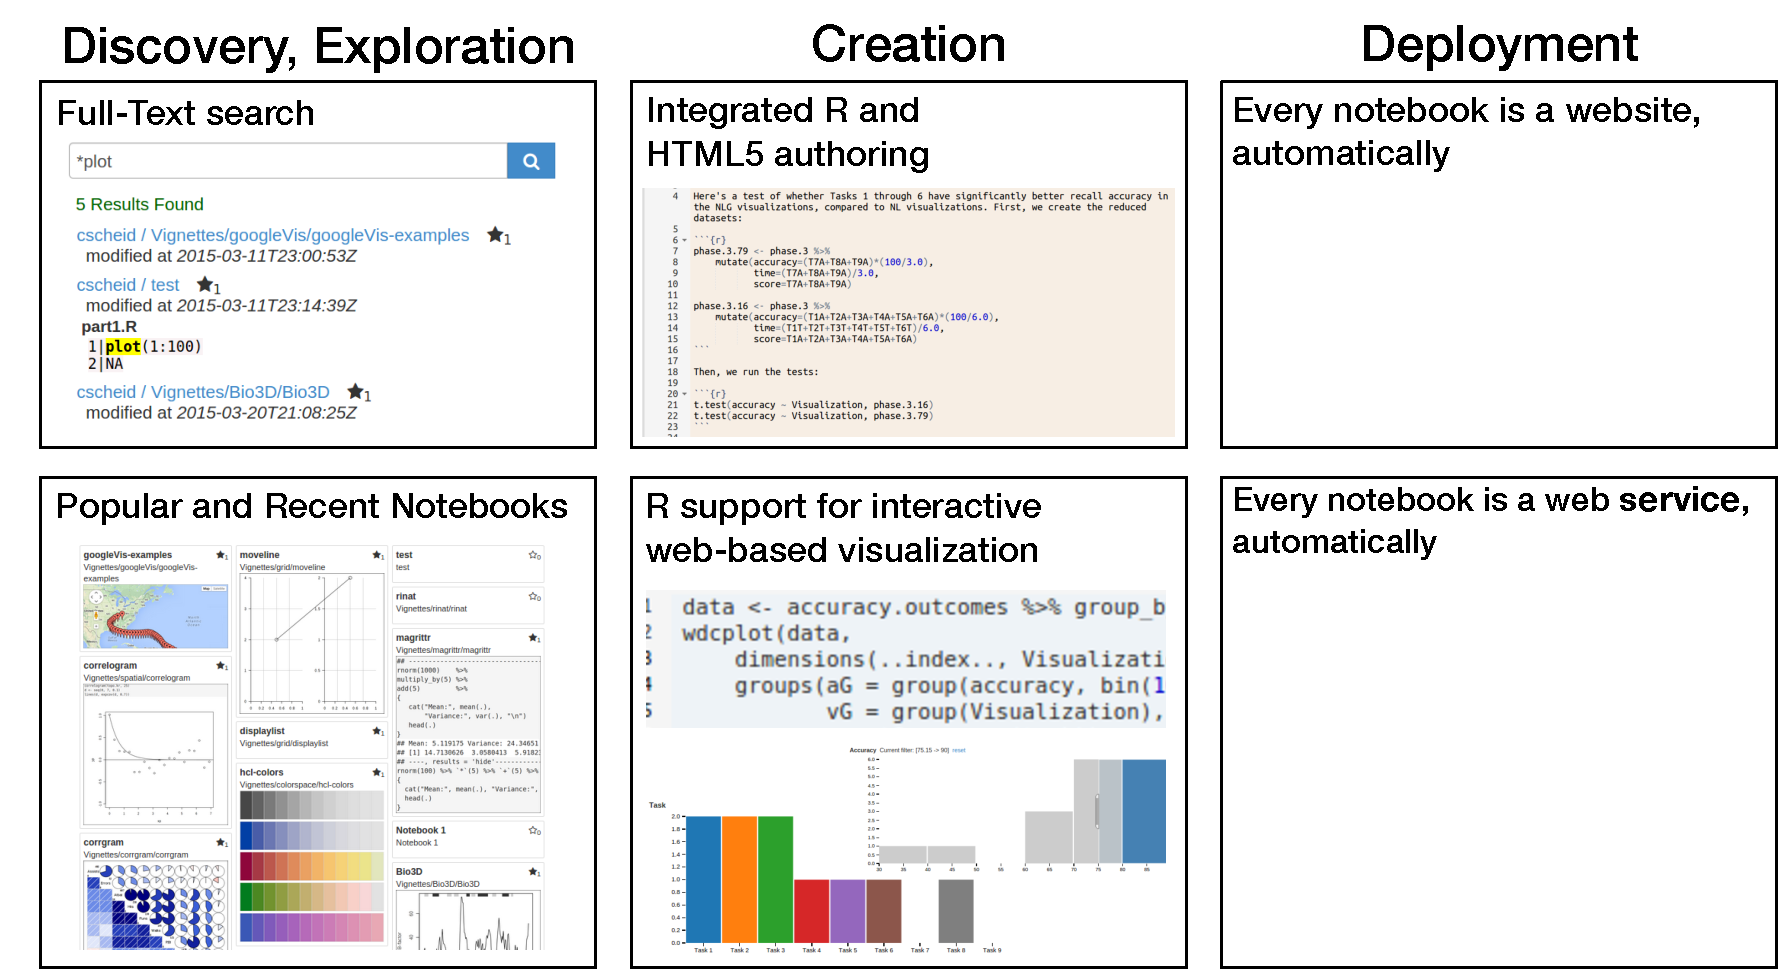
\includegraphics[width=.95\linewidth]{fig/teaser/teaser.pdf}
  % \vspace{-.5em}
  \caption{
    \carlos{Come up with caption for this. The story is: hackers/scripters work in the middle (and bottom-right), rest of organization has automatic access to their work on left and top-right.}
    \stephen{An overview of RCloud. a) Workbooks of published experiments and production applications are visible and searchable by all authorized users in an organization b) Data scientists create, publish and anotate workbooks with support for sharing and recommendation c) Workbooks can be parameterized and deployed as production services}
  }
% \vspace{-.5em}
}

%% Uncomment below to disable the manuscript note
%\renewcommand{\manuscriptnotetxt}{}

%% Copyright space is enabled by default as required by guidelines.
%% It is disabled by the 'review' option or via the following command:
% \nocopyrightspace

%
% Useful Macros
%

\newcommand{\eg}{e.g.\xspace} % e.g. and i.e. ARE NOT ITALIC!!
\newcommand{\ie}{i.e.\xspace}
\newcommand{\todo}[1]{\textcolor{red}{#1}}

\newcommand{\stephen}[1]{{\color{green} SN: [{#1}]}}
\newcommand{\carlos}[1]{{\color{cyan} CS: [{#1}]}}
\newcommand{\simon}[1]{{\color{red} SU: [{#1}]}}
\newcommand{\gordon}[1]{{\color{violet} GW: [{#1}]}}

%% \renewcommand{\stephen}[1]{}
%% \renewcommand{\carlos}[1]{}
%% \renewcommand{\simon}[1]{}
%% \renewcommand{\gordon}[1]{}


%%%%%%%%%%%%%%%%%%%%%%%%%%%%%%%%%%%%%%%%%%%%%%%%%%%%%%%
%%%%%%%%%%%%%%%%%%%%%% ALGORITHM %%%%%%%%%%%%%%%%%%%%%%
%%%%%%%%%%%%%%%%%%%%%%%%%%%%%%%%%%%%%%%%%%%%%%%%%%%%%%%

\renewcommand{\algorithmicthen}{}

% aux. commands

%%%%%%%%%%%%%%%%%%%%%%%%%%%%%%%%%%%%%%%%%%%%%%%%%%%%%%%%%%%%%%%%
%%%%%%%%%%%%%%%%%%%%%% START OF THE PAPER %%%%%%%%%%%%%%%%%%%%%%
%%%%%%%%%%%%%%%%%%%%%%%%%%%%%%%%%%%%%%%%%%%%%%%%%%%%%%%%%%%%%%%%%

\begin{document}

%% The ``\maketitle'' command must be the first command after the
%% ``\begin{document}'' command. It prepares and prints the title block.

%% the only exception to this rule is the \firstsection command

\firstsection{Introduction}

\maketitle

More than a half-century ago, Tukey foresaw
much of what is now commonplace in data analysis~\cite{TukeyFDA}.
Powerful, interactive environments for analysis and programming were
the goal, together with an unflinching (and, at the time, somewhat
heretical) insistence in keeping humans as a central part of the
discovery process. His now-famous quip that ``the picture-examining eye is the
best finder we have of the wholly unanticipated'' has come to define
much of visual analytics and exploratory visualization~\cite{TukeyEDA}.

In some way, we have moved far beyond what Tukey imagined:
computing and networking capabilities today far exceed
what was barely imaginable then. 
We argue, on the other hand, that we \emph{develop} our data analysis
solutions, and context in which they become part of the broader issues
being solved in organizations, has not changed as much: the S language
was developed essentially alongside Unix~\cite{TheSSystem}, after all.
We turn our attention to this opportunity to use computation
to support, not only individuals, but entire teams and their
work within larger organizations. In this paper, we contribute the
design of RCloud, together with an interview study conducted over the
course of its development and deployment at AT\&T Labs, where RCloud has
been in use for about two years.

Consider the role of a data science team within
a business or technical organization today.
Project teams vary in size, from just a few people to dozens or
more, even within one project's duration. Assignments are often
broad, and include tasks such as problem identification,
data wrangling, modeling, analysis, visualization, summarization,
presentation and interpretation of results, and recommending
actions to help clients to realize the benefits of the analysis.
Eventually, knowledge or working prototypes created by these teams
are transferred to other organizations to employ them in production.
There are many details to these tasks. For example, data wrangling can involve
finding data, understanding its syntax and semantics, assessing data quality,
performing normalization and data quality remediation, and making the data
available to other tasks that will follow.

Visual analytics depends greatly on communication and collaboration.
At almost every step, detailed knowledge about data, code and tasks
is shared by collaborators. 
Further, data scientists are increasingly asked to work more closely
with business or domain specialists who may be less technically oriented.
Thus, data scientists and developers are being asked to become
very broad, and integrate work across the spectrum.

%% Interviews in {\it Data Scientists at Work} by Sebastian Gutierrez illuminate
%% the teamwork and sharing in the current practice of visual analytics in industry.
%% We particularly appreciated the remarks by Jonathan Lenaghan about the potential
%% for continuous integration and publication.

%% % \begin{addmargin}[1em]{1em}  % left and right margin change
%% % part1.txt
%% Erin Shellman [of Nordstrom] described the benefits of
%% continuous deployment of experiments, and sharing knowledge
%% through software and data analysis artifacts.
%% ``Finally, prototyping our products so that internal
%% customers can use them early on has been crucial for
%% our success. It doesn't even have to be something
%% fancy. For instance, our recommendations preview
%% tool doesn't have a particularly interesting
%% visualization, but its enough to show the result of our
%% algorithms. Now we can shoot off a URL to internal
%% customers and it allows them to sit at their desk and
%% understand the behavior of our product and
%% experiment with it, and provide feedback way before
%% we're talking about getting it into production. This
%% has been super helpful and has been a really great
%% way to get people excited about what we're working
%% on...
%% %Building and maintaining those relationships are
%% %just like anything else-- you always have to be
%% %working on them. Nurturing those relationships are
%% %part of the job, and if you leave them unattended,
%% %they might not be there later.
%% %
%% % part2.txt
%% %Gutierrez: How do you share the knowledge you are
%% %building with others?
%% We’re obsessed with Confluence from
%% Atlassian, and the Data Lab has a very active
%% Confluence space. Recommendo is fully documented
%% on Confluence, so anyone in the company could learn
%% how it’s built, where to find it, and how to use it.
%% We also share exploratory analyses and reports on
%% Confluence so that we can still exchange knowledge
%% even if the work didn't make it into a larger project.''

%% % part3.txt
%% John Foreman commented on the scope of the work in
%% data science teams.
%% ``I lead the data science team at
%% MailChimp, and I like to get my hands dirty too.
%% Some of the big pieces of my day involve working
%% with my team to take stock of current projects and
%% figure out where to go next, doing my own work and
%% prototyping things-- I do projects just like my peers
%% do and then also my talking with other teams,
%% talking with management, and planning for the
%% future.
%% On our team, we've got different folks facing different
%% % part4.txt
%% kinds of projects. We've got one person who really
%% owns compliance and looks at our compliance
%% processes. We've got another data scientist who
%% focuses on more of the user experience side of the
%% house and understanding our customers. I help them
%% and others as is needed while I do the three things
%% mentioned earlier-- build data products, be a
%% translator, and have conversations with the data
%% science community.''

%% % part5.txt
%% Jonathan Lenaghan from PlaceIQ discussed to the potential
%% for continuous deployment in data science.
%% ``If you look at dev ops right now, they have things
%% such as continuous integration, continuous build,
%% automated testing, and test harnesses-- a1l of which
%% map very well from the dev ops world to the data ops
%% (a phrase I stole from Red Monk) world very easily. I
%% think this is a very powerful notion. It is important to
%% have testing frameworks for all of your data, so that if
%% you make a code change, you can go back and test all
%% of your data.''

%% % part6.txt
%% Anna Smith from Bitly spoke about the benefits of access to
%% a rich environment of shared data and code.
%% ``In addition to Bitly's extraordinary data sets,
%% I was given all the resources that I needed. These were
%% resources that I’d only heard about but had never
%% seen. I went from asking what a Hadoop cluster was,
%% as my school didn't have one, to being able to work
%% with one. Now I could play with one to figure out how
%% to make my work better and how to change my
%% algorithms so they were cleaner and ran faster on
%% Hadoop. The whole transition was eye opening. Not
%% only that, I could also look at other people’s code and
%% play with their code and data sets as well. It was
%% fantastic and I was convinced that working with data was my thing.''
%% % \end{addmargin}

%% % (Hiring ``full stack developers'' to perform integration seems to be a trend, but does not achieve the potential benefits of specialization and division of labor in larger teams, and is not a practice to be encouraged.)

Unfortunately, the processes and technologies supporting data analysis visual analytics are fragmented.
Knowledge is shared through informal conversations, emails,
meetings, phone calls, source code itself, in wikis, in project documents and
by other means. Results of experiments are often shared first by copying static
output (usually a simple screen shot or image output). By the time
decisions are made based on the results of that screenshot, the data
and the processes might have changed enough to bring to question the
original decision.

%% This disjointed, inconsistent process inhibits the use of tools to bridge
%% the many gaps and to help people find resources.
%% For example, even when code is shared, we still not may know where to
%% find examples that show how to use it.
%% When we find a useful data source, we don't know what packages or
%% other data sources usually go along with it, what problems with the data
%% others have already discovered and corrected, or where to obtain online feeds
%% to get updates.

This situation can affect how data science teams; as analysts and
toolbuilders, we have experienced this first-hand in our environment, and
others report similar findings. Gutierrez collected interviews with data
scientists~\cite{Gutierrez:2014:DSA}, which include the following:

\begin{itemize}
\item (upon being given access to other code and data analysis, in
order to learn about Hadoop) ``[...] Not only that, I could also look at other people’s code and
play with their code and data sets as well''
\item (discussing the value of sharing prototypes rather than static
data) ``[...] Finally, prototyping our products so that internal
customers can use them early on has been crucial for
our success. [...] Now we can shoot off a URL to internal
customers and it allows them to [...] provide feedback way before
we're talking about getting it into production.''
\item (on sharing more than just a finished product) ``We also share
exploratory analyses and reports [...] so that we can still exchange
knowledge even if the work didn't make it into a larger project.''
\item (on changing analyses and processes) ``It is important to
have testing frameworks for all of your data, so [...] you can go back and test all
of your data. 
\end{itemize}

Currently, these concerns need to be addressed \emph{alongside} the
visual analytics environment. Some symptoms of the current situation are:
\begin{itemize}
\item It is hard to find data, metadata, and knowledge about them.
\item Most coordination is done through meetings, whose content is not related to other artifacts and may not even be stored.
\item Production deployment requires porting code to a different environment or even completely rewriting it, thwarting continuous release.
\item Many tools adopt a standalone or single developer perspective,
not suited to collaboration and web deployment. 
\item Analysts find insufficient support for tracing events or issues from production back to the EDA process.
\end{itemize}

In view of the opportunity to improve this situation,
we created a software environment that supports the end to end
visual analytics process for individuals and teams.
This environment knits together some familiar tools, and 
provides new features to find data and code; create experimental workbooks;
run experiments; annotate and deploy experiments as end-user websites or
as reusable, callable services; and to share, search and recommend these artifacts. The artifacts are stored in a version
control system that provides a common workspace, as well as needed control
and isolation between stable and experimental versions of code and other
resources. 

A key point is that, for the most part, the improved capabilities are
available by default, without much explicit intervention on the part of
data scientists and other customers. Visual analytics experiments are
conveniently shared and turned into production websites, without moving
or porting code. All the published artifacts in the system can be
searched immediately. Recommendation is as easy as clicking a star
on a useful workbook.

The high level architecture of the prototype system
is shown in figure~\ref{fig:high-level-architecture}.
We chose R as the foundation for our prototype because it is already
the dominant statistical computing language in our lab.
R also has many useful packages for data analysis and visualization,
and the core system and its packages are open source that can be modified to
support research. 

From a more principled or theoretical perspective, visual analytics goals
or objectives for emerging systems, described in previous work, closely match
the goals of our prototype. Adopting the terminology of X Y and Z, we noted
the following.

\begin{enumerate}

\item Technology transfer.
In most organizations, development of analyses and visualizations 
s done by \emph{hackers} and \emph{scripters} (adopting Kandel et al.'s
terminology~\cite{Kandel:2012:EDA}). \emph{Application users} 
gain the benefits of the tools developed by hackers and scripters.
Generally, the connection between these two worlds is made by IT staff,
who port or even rewrite code so it can run as a stable production service.
In an environment where business needs can change rapidly, this
process does not scale. Our objective is to merge the worlds
of EDA and production.

\item Coexistence. In the current data science ecosystem, the
isolation of exploratory visualization and data analysis
environments hinders wider adoption of modern techniques from each.
The richness of interactive visualization tools is still somewhat
separated from the power of statistical programming environments.
There is an opportunity to provide a framework so that developments
on each side are more easily adopted by the other, and made available
in production services.

\item Discoverability. A chronic complaint of data analysis teams is
repeated work (``How can I connect to database X?'', ``How do you get
clean data from column Y from feed Z?'') This work arises from lack of
communication about previously solved subproblems. Our goal is encourage
and support transparency of work between team members.

\end{enumerate}

Over the past three years, we prototyped RCloud and deployed it to
a community of data scientists, business analysts and other colleagues.  The
platform today has over 300 active accounts; about 20 people use it regularly,
another 30 people use it more than once a week, and another 50 use it more than
once a month.  Most of the
active users are members of AT\&T Labs, but some are data scientists and other
collaborators in other business units.

\carlos{we need a segue into related work}.

\begin{figure*}
\centering
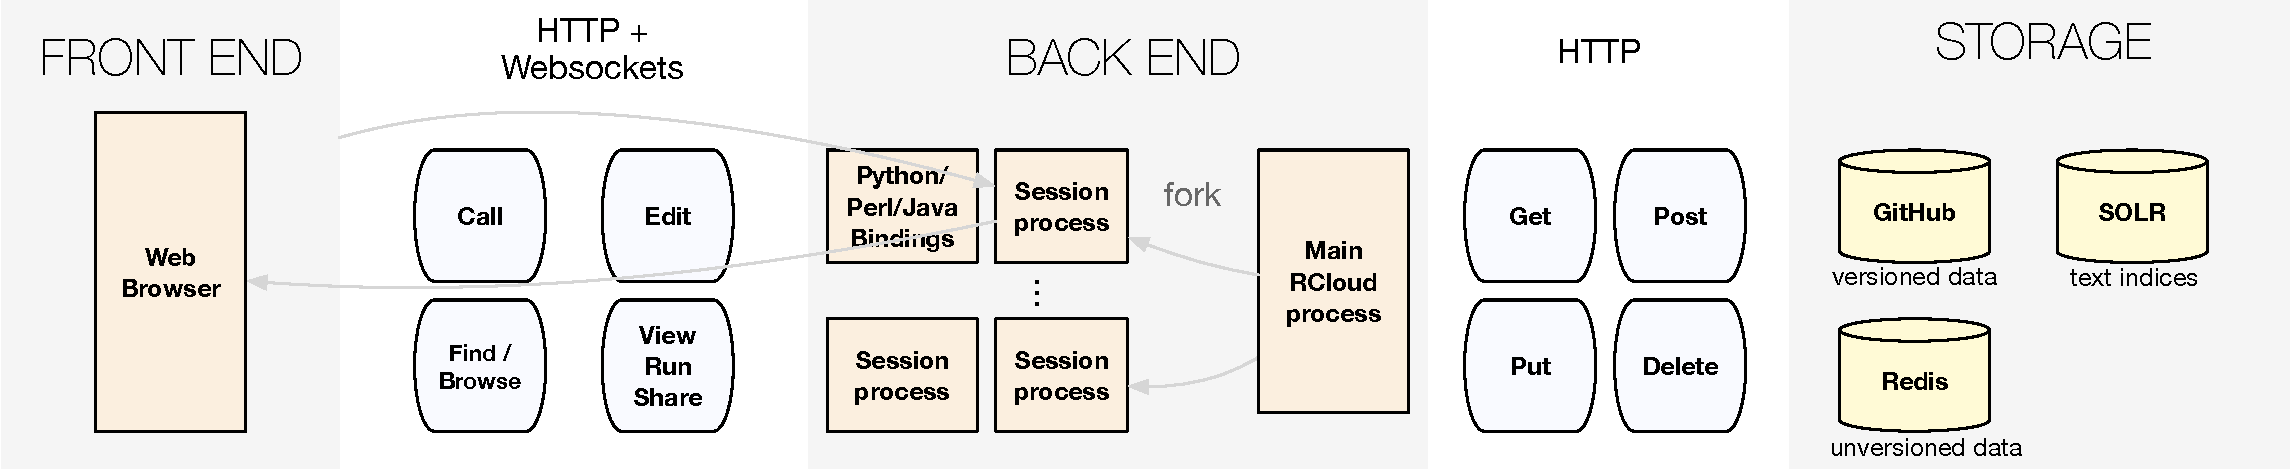
\includegraphics[width=.75\linewidth]{fig/system/system.pdf}
\caption{\label{fig:system}A diagram of RCloud's architecture. }
\end{figure*}

\section{Related Work\label{sec:related}}

Broadly, the entire field of information visualization and visual analytics
revolves around improving how users solve problems involving data.
In this section, we focus specifically on
system work relating to problem-solving environments and multiple users.

\paragraph*{Social Data exploration and Analysis}
ManyEyes~\cite{Viegas:2007:MAS} was a landmark system designed
for the crowdsourced creation and publication of data
visualizations. Although ManyEyes only supported a limited number of
visual encodings, the system's success was both a precursor to more
sophisticated solutions and an early indication that the world-wide
web was a suitable platform for data visualization. One of the main
challenges we faced in designing RCloud was providing an experience
for \emph{consuming} visualizations as seamless as ManyEyes's, while
sacrificing as little as possible on the generality of the analyses
themselves.

\paragraph*{Notebooks as a medium for data analysis dissemination}
The concept of a ``notebook'' as we use it here can be traced all the
way back to Knuth's literate programming~\cite{Knuth:1984:LP}. In
literate programming, a comprehensive description in prose of the
behavior of the program is ``weaved'' together with the source code,
yielding both an executable program and a human-readable document.
A notebook represented as a collection of short, executable cells,
originated with Mathematica, and in R, literate programming is
supported by packages such as knitr and RMarkdown~\cite{Xie:2013:DDW}.
Project Jupyter~\cite{jupyter} (originally implemented as part of
IPython) offer some notebook features, but lack a transparent
mechanism for sharing and deployment in multiple-user settings.
%
Further afield, {Electronic Lab Notebooks} are applications for organizing
and sharing data from scientific lab experiments\cite{Rubacha:2011:ELN}.
In a sense, we hope to adapt and extend this concept to the work of
visual analytics teams.
%
Although RStudio offers publication of literate R programs as a free
service on their website, the workflow is somewhat disconnected from
the development of those programs. Once they're uploaded, it's hard
for other users to build off of the work published (or even for the
original author to update new versions). In other words, RStudio
handles \emph{publication}, but not \emph{deployment} and sharing.

\paragraph*{Provenance and versioning} As
mentioned, one central issue in exploratory analysis is that
problems change quickly over time, often in the course of developing a
solution. As a result, systems should provide adequate support for
tracking \emph{changes} of the data analysis scripts. VisTrails was
one of the original systems for managing \emph{process provenance} ,
and demonstrated the value of capturing aspects of the processes that
surround data analysis experiments and tools, including detailed
history, collaboration, and deployment~\cite{Callahan:2006:VVM}.

VisMashup~\cite{Santos:2009:VST} defines a schema and
semantics for automatically deriving user interfaces from workflows,
while Crowdlabs exposes these capabilities on a website
feature~\cite{Mates:2011:CSA} workflow upload and remote execution. In
our view, the impedance mismatch between a dataflow pipeline
specification and the power of a general-purpose language is too great
for the type of general exploratory work in data science teams. At the
expense of ease of use for non-programmers, RCloud tries to provide a
closer match for analysts accustomed to creating and executing R and
Python code, while retaining attractive properties like transparent
provenance tracking and interactive data visualization on the web.

\paragraph*{Web-based tools for sharing code snippets}
There have been quite a few tools recently developed for quickly
sharing small programs on the web, including
bl.ocks~\cite{blocks}, jsfiddle~\cite{jsfiddle}, and
plot.ly~\cite{plotly}. bl.ocks and jsfiddle are designed to
share Javascript programs, which means that deployment happens
automatically through the web browser. If Javascript eventually becomes
the lingua franca of exploratory data analysis, we can foresee
building a simpler version of RCloud where all execution happens
either on the client side or via web services. Unfortunately that is
not a realistic assumption at present, making these stand-alone
solutions unsuitable for our purpose. Plot.ly is notable in that it
provides API support for publishing \emph{from} scripts: in other
words, it is possible to generate a plot.ly visualization from inside
another program. Although this is an intriguing idea, it
nevertheless creates a disconnection between the analysis and the
resulting visualization. In RCloud, we wanted to ensure that every
visualization is transparently linked to the source code that
generates it.

%% publishing web content such as knitR, Rpubs,
%% rCharts, and gg2v. These tools are not collaborative, but they are
%% aimed at better graphics and web applications.
%% . {\bf iPython
%%   notebooks (Jupyter)} are the closest work we are aware of.  The goal
%% of this project is to provide shared notebooks and a remote execution
%% environment for interpreted scripts.  \stephen{Are there significant
%%   differences involving versioning, provenance, annotation and other
%%   broad process support?}


%% {\bf bl.ocks, jsfiddle, plotly} and other web services for sharing code
%% and demos.


\paragraph*{Needs of data analysts}
Kandel et al.'s interview study points out the typical ``explore'',
``model'', ``report'' cycle in enterprise data
analysis~\cite{Kandel:2012:EDA}. There are many discontinuities in
this cycle that cost time and effort to overcome. RCloud seeks to
reduce this mismatch. Kandel et al also point out that larger teams
are becoming more common in data analysis, that supporting
collaboration is difficult and important, and that sharing
and versioning of data sources and artifacts is hindered by current
technology. ``We found that analysts typically did not
share scripts with each other. Scripts that were shared were
disseminated similarly to intermediate data: either through shared
drives or email. Analysts rarely stored their analytic code in source
control.'' Their study highlights the opportunity for better ways
of supporting collaboration and sharing in data analysis teams.

An earlier study by Kandel et al argues that data wrangling
(cleaning, parsing and transformation)is a major part of exploratory
analysis and visualization~\cite{Kandel:2011:RDI}. We view this
as attacking a different semantic level than ours, but also
showing the need for an environment that enables better sharing
of the knowledge, tools and processes to do this. Anecdotally
we find much frustration among practitioners that this knowledge
is difficult to find and often is not recorded or available in a
reusable form even within the same organization.

Heer and Agarwala identify many design considerations for
collaborative visual analytics~\cite{Heer:2008:DCF} that
influenced our work.
RCloud notebooks, and the integrated version control system for them,
described in Section~\ref{sec:notebooks}, address modularity and granularity,
and artifact histories.
\emph{Starring}, the means for signaling interest in notebooks, described in
Section~\ref{sec:starring}, addresses social-psychological incentives,
recommendation, and voting and ranking. RCloud's integrated deployment
mechanism, described in Section~\ref{sec:deployment}, addresses the cost of
integration, content export, presentation and view sharing.

The need for integrating statistics and visualization has been
highlighted in previous studies and is widely understood by
various technical communities \cite{Perer:2008:ISA}
Lucas and Roth were early advocates of combining
data exploration with presentation and publication \cite{Lucas:1996:EIV}.

There has been noteworthy work on specific techniques
to support collaborative or social code development and data analysis,
such as social bookmarking \cite{Millen:2006:DSB} \cite{Heer:2007:VAV}
and crowdsourcing \cite{Fast:2014:ECS}.
Similarly, there are computational methods to support high
performance execution in incremental code development
environments \cite{Guo:2010:TPI}.
The goal of RCloud is to define an environment in which many such
techniques may be integrated and made available to a broad community.
\begin{figure*}
\centering
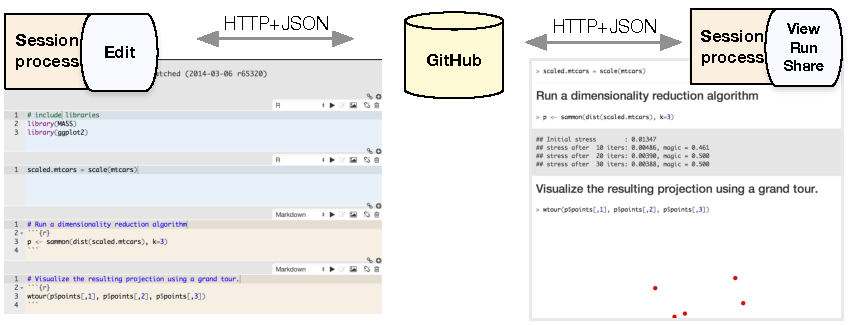
\includegraphics[width=.95\linewidth]{fig/notebook/notebook.pdf}
\caption{\label{fig:notebook}An RCloud notebook is a sequence of
\emph{cells}, each a snippet of source in one of the supported languages (typically R, but Python and others are also supported) or Markdown. The main creation workflow involves editing notebooks, which are transparently stored as git repositories in GitHub, providing us with easy access primitives for version tracking. Notebooks can be executed as they're edited (left), or in a standalone viewer (right), via a slightly different URL. This provides a lightweight, low-friction mechanism for sharing results which we discuss in detail in Section~\ref{sec:interviews}. }
\end{figure*}

%% \stephen{We have a problem we already went over some of this.}
%% Our work has been inspired by and benefited from other efforts
%% to improve data analysis environments and processes. Building in
%% the immense foundation of systems for statistical graphics,
%% recent work includes RStudio \cite{RStudio:2013:SWA},
%% the R packages Markdown \cite{Allaire:2014:MMR},
%% knitr \cite{Xie:2013:DDW}
%% and Shiny \cite{RStudio:2013:SWA},
%% and iPython notebooks \cite{Perez:2007:IAS}
%% to name a few. RStudio aims at providing an integrated development environment
%% for R, with support for publishing code in packages. Markdown,
%% knitR and Shiny augment R with sophisticated reporting capabilities, including
%% interactive web interfaces. IPython \cite{Perez:2007:IAS}
%% shares many of our goals, such as providing a comprehensive environment
%% for analysis and programming, and share-able documents on the web.
%% \stephen{Do we now need to introduce one of those remarks where we
%% explain that we are not the same as IPython.}

One overall goal is to reduce the gap between implementers and
deployers in visual analytics. The fusion of development with
production operations in software release management (``DevOps''
\cite{Httermann:2012:DD} or ``continuous integration''
\cite{Fowler:2006:Continuous}) is a trend in web services and similar
fields. By making it convenient for data scientists to expend just a
little additional effort when creating experiments, we may be able to
eliminate the need for programming teams to recreate their work to
deploy it in production, which has a high cost in time, expense and
accuracy.

We next give a description of the system architecture,
and how it enables capabilities that satisfy the requirements as described.

\section{The System\label{sec:system}}

\subsection{High-level Architecture\label{sec:highlevelarchitecture}}

% Stephen: Let's work from front to back, from human interface to the
% services and frameworks that support it.

The internal computing infrastructure of organizations has changed
radically in the last fifteen years. The shift from large
servers toward scalable, lower-cost, distributed systems (``the cloud'')
led to a software ecosystem of processes distributed over a
network, usually communicating via HTTP. HTTP is dominant because
web browsers and servers are ubiquitous and available in almost
all hardware devices, from tiny sensors, to handheld devices and
laptops, to rack-mounted servers.

As a result, HTTP is the lingua franca of interprocess communication
(IPC). One of the design goals for RCloud was to provide a productive
environment for creators of data-analysis scripts, that also behaves
as a first-class citizen in the pre-existing ecosystem of computer
services and networks in an organization.

%% Design for cloud-friendly? This goes back to the point in the
%% introduction about playing nice with the rest of the ecosystem.

\subsection{Human Interface\label{sec:humaninterface}}

%\stephen{What??}
%We designed RCloud around the front-facing API, which provides roughly
%one entry point to correspond with each requirement.

Figure~\ref{fig:notebook} shows the RCloud developer interface.  The center
panel is a notebook for code and visualizations.  Code is edited in this panel,
and visualizations are rendered.  An inventory of supplementary ``asset'' files,
that are part of the notebook, though not in its executable flow, are edited on
the right.  Controls at the top of the screen allow the user to run, view, and
share the notebook. \gordon{Why are we talking about the callable interface
here?} The result of code execution is the final cell of the notebook.  On the
left is a browsing area for searching and viewing other users' notebooks, and a
help system.

The call mechanism is the URL itself; arguments are read from the URL
and the final cell is rendered as the result.

\subsection{Notebooks\label{sec:notebooks}}

The main unit of computation in RCloud is a \emph{notebook}.
A notebook holds a sequence of \emph{cells}, each of which contains a
snippet of code or hypertext in Markdown. This is not a novel idea;
executable documents structured this way are a feature of many
other systems, including Mathematica, IPython and Sage.
\stephen{Code is executed when...?}

One of the main contributions of RCloud is the idea that notebooks
are ``always deployed''. In other words, the most recent version of
a notebook is immediately available.\stephen{What if it is broken?}
This makes it convenient to share and modify experiments and compose
results without binding to a specific version of a notebook.
On the other hand, there are situations where it might be important
to name specific versions. We do not expect designers to decide which
versions need to be preserved, but we embrace \emph{transparent} versioning.
This is similar to models like Jankun-Kelly et al.'s p-set calculus \cite{Jankun-Kelly:2007:MFV}
and VisTrails's version tree \cite{Callahan:2006:VVM}, where every change in the state of the system is tracked.

To implement this, we built RCloud on top of GitHub's \emph{gists}~\cite{GitHub:2014:GG}.
GitHub offers a HTTP interface for creating simplified git repositories, the main limitation
being a restriction to text-only files in a single directory. The GitHub web-service
API provides most of the semantics we need for the versioning portion of the storage back end:
access to previous versions, comments, starring, and forking.

Using GitHub for storage and versioning also exposes other capabilities
that can be invoked with JSON and HTTP.
Particularly, we can provide full text search using Apache SOLR.
SOLR is scalable, can index in near-realtime, supports multiple character sets,
indexes several common types of documents, and has schemas and faceted search.
%
Integrating existing services and software components, especially open source,
instead of implementing custom code is a trend in the software industry, and
is very positive for systems research and prototyping in visual analytics.
By adopting existing technology, small teams with limited resoures can explore
novel ideas toward the improvement of large, complex software ecosystems.
In our case, even though this approach involved learning standards not directly
related to visual analytics, our early decision to use the GitHub Gist API
turned out to be successful. Future projects could gain many of the same benefits
by adopting this strategy. In fact, it will be essential for technology adoption
and transfer, because it is almost impossible for any one tool or platform to
``own'' or support the entire visual analytics process.
\stephen{Are we preaching too much?}

\subsection{Reputation and Interest: starring\label{sec:starring}}

Information retrieval based on collecting usage and recommendations
is a cornerstone of modern web services. We would like to help data
scientists to find workbooks (and therefore items in their contents
such as code, data, and colleagues with specific expertise) with
the benefit of such information.

In RCloud, reputation and interest are a relationship between
\emph{notebooks} and \emph{users}, rather than a relationship between
user pairs. We chose this approach because we expect initial 
RCloud deployments to have relatively few users, but some users to
create many notebooks. Under that assumption, assigning interest
to users would not provide sufficiently ``high-resolution'' data.

We incorporate both explicit and implicit indications of interest
in notebooks. Explicit interest is indicated by ``starring,'' or
clicking on a button that marks a notebook as interesting.
This makes explicit indication of interest a nearly trivial operation,
always readily available, to encourage its use.

Implicit signaling of interest is supported by keeping click-through counts
\cite{Joachims:2005:AIC} and execution counts. (In addition to these
standard techniques of collecting feedback from web search, we anticipate
applying static and dynamic code analysis to infer fine-grained
information about relationships, for example, which packages and data
sets often appear together.)

\subsection{Executing R in a web browser\label{sec:Rinbrowser}}

One our main goals is to provide ubiquitous access to the statistical
tools of the R programming language in the wider environment in which data
science teams participate.
%
Given the recent developments of interactive visualization and visual
analytics in HTML5 and the web, we decided to create an
\emph{interconnect} between the two environments.
%
Every RCloud session spawns a new R execution process in a remote
server.

%% \subsubsection{Object capabilities: R to Javascript RPC and access
%%   control}

HTTP and web services are convenient but much of the protocol is
stateless. (For example, GET requests are required to not change the
remote state, and results can be cached in transparent proxies along
the network). In the case of close communication between a running
R process and a web browser, we need something that is more flexible
than distinct URLs for every R process, and which embraces
statefulness of both calculations and visualization parameters.

\carlos{In-depth explanation of R<->web interconnect, and why it's
  necessary or important. Main point: make programming in the R side
  as close as possible to what R programming feels like, and make
  programming in the Javascript side as close as possible to what
  Javascript programming feels like. We do this because this part of
  the system is targeted at programmers; Shiny targets web programming
  at non-web-programmers. We don't attempt such a thing and land at a
  different point in the spectrum.}

\carlos{compare against https://www.opencpu.org, compare against
  IPython notebooks. Two-way communication? Actually describe what it
  is. IPython manipulate notebooks? Understand and contrast}

\subsection{Interactive notebooks\label{sec:interactivenotebooks}}

%% How do we do things that are not trivial to do with IPython (for
%% example)

%% What is relationship to a standard CMS with R/Python

%% dcplot. two-way communication between between backend session and
%% frontend session.

A key engineering decision in RCloud was to rely on full two-way
communication between the web client human interface, and data and
computing resources in the cloud. It is easier to engineer a design
in which the human interface is pushed one-way from the server
and thereafter all interaction takes place within the client.
Two-way communication is necessary, though, where the size of
the data or computational performance makes it impractical to
move all computation to the client.

In addition, R is well suited as a language for analysis, and
JavaScript for interactive visualization. To draw on
the strengths of both languages and both environments, the connection
between the languages is not just procedural: it makes \emph{closures}
and \emph{first-class functions} available across the network.
This provides considerable flexibility, so that for example, a chart built
with dc.js or leaflet.js can call back to analysis functions in R
without having to formalize the protocol between the processes.

\subsection{Deployment of notebooks\label{sec:deployment}}

Every notebook in RCloud is named by a URL, and notebooks by
default are visible by the entire organization. This is deliberate.
As pointed out by Wattenberg and Kriss~\cite{Wattenberg:2011:DFS},
broad access to analysis outputs (in their case, for NameVoyager)
increases long-term engagement in part through cross-references on
the web. Although our prototype RCloud deployment is only visible
inside a corporate intranet, we nevertheless found anecdotal support
for this notion by discovering links to RCloud notebooks in internal
discussion fora and mailing lists.

Because notebooks are continually published, any work is immediately
available both as a subroutine and a visual component. Close colleagues
can start on the next stage of analysis, or delve into the data,
even while the original author is polishing an algorithm or its
presentation. \stephen{We glossed over the things that can go wrong.
We should at least discuss that briefly.}
The code is the page, and can either be shaped into
a function of inputs and outputs, or the linear cells of the notebook
can be reworked into a full-fledged HTML layout.

\section{Case Study}

To illustrate some aspects of RCloud, we present an example application
for stock price analysis.\footnote{Unfortunately this report could not
include production notebooks containing proprietary or personal information.}
The example, although simplified, shows key steps in the development
and deployment process we support.

\begin{figure}
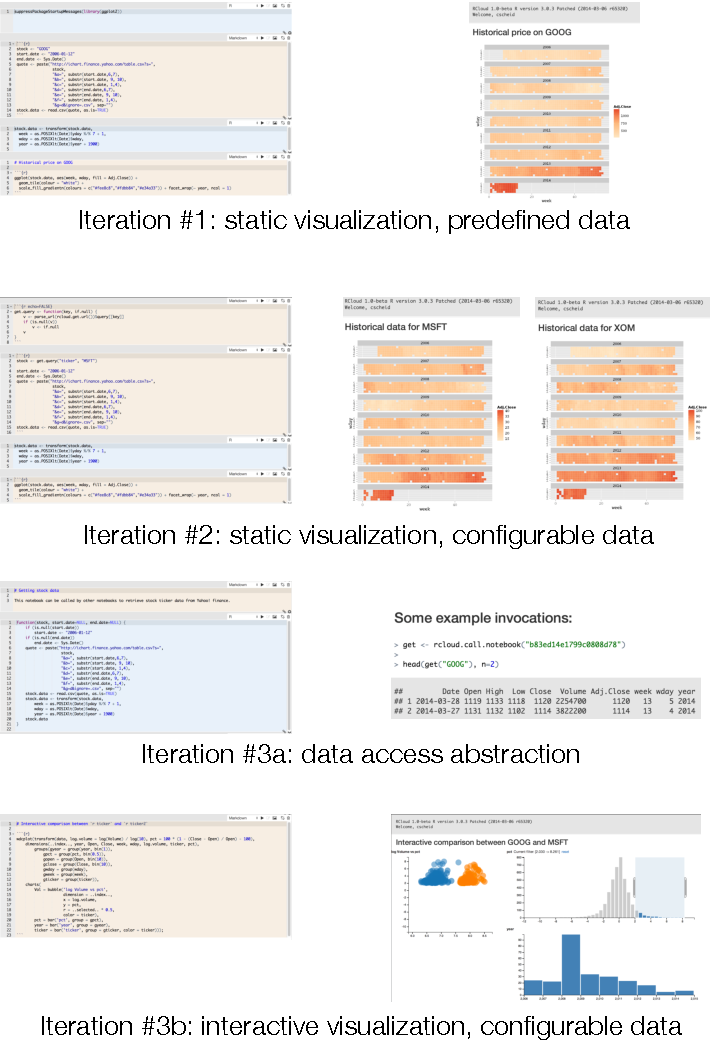
\includegraphics[width=\linewidth]{fig/casestudy1/casestudy1.pdf}
\caption{\label{fig:stockvis}Iterations of a stock ticker
  visualization, based on an example by Hadley Wickham. A
  simple, static visualization of the closing price of a single stock
  is progressively developed into a configurable display suitable
  for dashboarding, then into an interactive visualization for 
  comparing the volatility and volume of two stocks, and finally
  into an API for data access by other RCloud notebooks. The notebooks
  in this example can all be loaded as web pages. When a notebook
  corresponding to a function call is displayed a web page,
  its associated documentation is displayed.}
\end{figure}

It shows a sequence of visualizations of the performance
of financial stocks over a multi-year period. The first visualization
in this example uses ggplot2 and was written by Hadley Wickham.
It reads data provided by Yahoo! Finance as a web service, and shows
the price for a single trading symbol.

The webpage that produces that visualization includes a link back to
the underlying source code. From this link, a user can fork the notebook.
In the example,a configurable ticker is added, based on the URL of
the notebook. The change to the notebook is very minor.

Next, the notebook author or a collaborator may decide to extend
the application to also provide convenient access to the data,
apart from its visualization.
This is done by creating a notebook that defines a function.
That notebook then becomes a \emph{subroutine} for other notebooks.
It can be invoked from interactive notebooks, such as dashboards.
The data access notebook is version-controlled like other notebooks.

Finally, consider the situation where an analyst wants to understand
the price dynamics of stocks with respects to various attributes and
time ranges. For this, interactive visualization may be very helpful.
In our example, the analyst creates an interactive tool with multiple
linked views.

Through the tight integration of R and JavaScript functions and data,
the analyst writes a function in R which passes the dataframe and the
description of the charts to the dcplot library.  Simple R expressions
are captured as trees to generate JavaScript expressions.  The terse
chart description language, with intelligent defaults inspired by
ggplot2, provides a simple yet powerful interface to the grouping
and reduction functionality of the well-accepted charting libraries
crossfilter, dc.js and d3.js.

% \subsection{Text analysis\label{sec:textvis}}
% Same.

% IMPORTANT: what is unique about RCloud here
% From prototyping to dashboard
% Getting other information from the web
%

\section{Interview Study\label{sec:interviews}}

To evaluate the effectiveness of RCloud, we interviewed 13 current or
recent users of RCloud. 9 are data analysts, and 4 build tools for data
analysts and business needs.

The subjects differed in their evaluation of its benefits and disadvantages,
as described below.

%Analysts were more annoyed by the cell interface and its perceived
%slowness than were web/tool developers. Analysts
%switching to R from another language were more likely to use RCloud for
%exploratory data analysis. Web/tool developers were more likely to see the
%need for parameterization.

\subsection{Sharing of results}
Sharing of notebooks is the core feature of RCloud, and a popular one. All
the subjects praised this feature.

%% Wendy's usage is typical:
%% \begin{quote}
%% I've been sharing my notebooks in order for other people to see what
%% I've done. It's very convenient for that purpose. [...] We haven't
%% been editing them together, but we've been just sharing, and I've been looking
%% at things that other people do. So there's no collaborative aspect of it, like
%% developing the code, but there's sharing aspects for other people to see and for
%% me to see other people's notebooks.
%% \end{quote}

By default, all RCloud notebooks are publicly visible, and notebooks can be
found by navigating the notebook tree, or by searching. However, users most
often mentioned sharing by sending links through email. Lilo says,
``If my supervisor wants to see what I've done or QA it, I can just send her a link.''

Besides providing a way to present work, notebook sharing can provide a
starting point for coding. Lilo says, ``The best part is how easily you can
share code. You can find a working example, rather than wearing
out Google and finding questionable examples that may or may not work.'' Wendy
notes, ``[If] some person has done something similar, then you're able to just
edit that, and that's saved a lot of work time for me.''

Evelyn develops packages for analysts, and uses RCloud ``more for sharing code with
other people, and for doing tutorials for {\em iotools} or {\em hmr}'', his packages.
``I want people to see how the package works, so I clearly want them
to see the code... I write it just like I would write GitHub
Markdown, where you have little code snippets and text, but RCloud lets me
actually run the snippets [and display the results].'' He also uses RCloud for
describing and debugging  problems with data sources.

Some users, who tried RCloud and were not able to continue for organizational
reasons, miss certain capabilities. Leith ``[likes] the concept of being
able to create notebooks and share them... A wiki is not the best way for
communicating results - it's kind of like writing a blog post with very limited
functionality. I have to save every picture and post it as an image.'' She said,
``I can't share all of the code because it would just get crowded and wouldn't
look right on a wiki.'' Iris explains, ``If I could make a folder on RCloud and
have Python notebooks and also Pig notebooks there, and execute them from RCloud,
that would be much better than my current [environment], because that would free
me from manual documentation and version control and also telling people where
my code was. It would be just, hey, go look on RCloud, here's the stuff.''

%% Kaylee: ``being able to share notebooks or codes, or collaborate on something,
%% easily being able to share that information. That's an obvious advantage and
%% nice to have.''

%% Kenyon: ``I like being able to look at other people's notebooks.''

\subsection{Forking}
The ability to start work where someone else let off, by forking, proved to
be a popular feature. In fact, almost twice as many (131) users have forked
someone else's notebook as have starred one (75).  Lilo says, ``It's one of the
handiest functions, because instead of having to find it, copy, paste it, you
just hit Fork, rename it, and it's done. It's pretty amazing.''

Although we intended forking to be available to improve others' code, we 
initially didn't anticipate support forking one's own notebooks, which
proved very useful. Kenyon says, ``I fork my own notebooks because I'm going off
and doing some other analogous project, so I've got interesting content that I've
already done in a previous analysis, that I want to start from and then tweak
to match a new set of data.''

Forking also provides a way for others to troubleshoot when something goes
wrong.  When Hugh works with the users of his notebooks, ``I'll teach people
to intercept the result in the middle, to insert print statements here and
there and check values.''

%% ``a lot of the time we just
%% insert print statements here and there and check values. Having debugging code
%% inside a functioning program is helpful for others to understand what
%% you're doing.''

%% Leith: ``gives the audience a way to try their own analysis, like maybe Leith
%% should have used this parameter and they can just change the parameters''

A common but somewhat problematic use of forking is to change
parameters. Wendy says, ``I've been forking other people's notebooks [because] I
want to run them on a different part of data, or I want to change some parts,
I don't want to see this column, I want a different column, things like
that.''  Evelyn complains that a notebook might say ```This is a report of
the volume of all of our feeds for this month', and someone would want to
look at it for the next month or the previous month, so they'd fork it to
change the month.''

Parameters can be added to a notebook URL, but adding user interface
elements to do the same thing requires expertise. Tool builders see a
need for facilities to make it easier. Allison calls it ``web-enabling'' the
notebook: ``[users] can always fork the notebooks and make changes, but I
feel that if the owner of the notebook web-enables it, it's easier to
run. Instead of forking it, if they can set options, it's probably more
efficient, and they can [still] fork it if they want to.''

%% Lilo: ``For the things that I'll do multiple times, I'll try to parameterize
%% it, and I'm working now on putting some packages together that will operate in
%% some fashion outside of RCloud, straight from the command line''

\subsection{Automatic source control}
%% Kenyon: ``when I've finished something, there's a nice clean record of it.''
%% (I think this may be more about the publish/markdown than about source control.)

Automatic source control is also a popular feature. Lilo says, ``Instead of
looking back and saying I've got a billion files here in this subdirectory and I
hope I've got them backed up, if they're on RCloud I know they are.''

%%  [...] I
%% don't have to worry about it, if I drop my computer in the bathtub, everythings
%% gone, because I'm not great about uploading my own for versioning.''

Iris points out that the automatic versioning works well for dealing with the
minutiae of web development:
\begin{quote}
I like the fact that it has a built-in editor, so
if you need to fix a typo in a link, or an extra line break or other
nonsense, you can just switch to the edit view, pull up your asset, type
something, it's automatically saved, committed, everything. You don't have to go
back to your source code, change it, commit it to the repo, pull the repo to
your distribution version. 
%% None of that's necessary. A lot of web development is
%% fixing stupid little bugs, and you can do that instantly without a lot of
%% overhead, which is nice.
\end{quote}

On the other hand, saving every change leads to many fine-grained
versions. Kenyon says that for this reason, the history feature is not that
helpful: ``I don't need something that keeps track of every mistake I've made or
every direction I've tried.''
%% Tagging these versions with names wouldn't
%% necessarily help because ``namespaces are already crowded, so trying to remember
%% the names of notebooks is hard, much less the names of states within each
%% notebook.''


\subsection{Discovering others' work}
Many users find the search function valuable. Wendy says, ``The fact that we have
all the notebooks there, searchable, saves me from replicating what other people
have done.''

But other users prefer to browse just the notebooks of experts they
know. Kenyon says, ``Usually I know somebody's notebooks that I want to search
through, because I know that the kind of thing I'm looking for is something
more obscure than I'm likely to find in some random person's.''

More selective ways to search will be needed as the number of notebooks
grows further. We explore some ideas in Section~\ref{sec:discussion}.

\subsection{Integrated analysis}
Integrating an analysis language into a web development environment is something
tool developers really appreciate.  The structure of Hugh's visualization
notebook means
\begin{quote}
the other guys who want to do analytics on the data can first pull
the data, do the analytics on it, and then feed the viewer the data.
Anyone from the stats group can insert something in between.
Once you get the data into RCloud, then you have a dataframe
to work with, and then they can produce another dataframe.
\end{quote}

Integrating R also helps Allison's application: ``Having an open session where I can run R commands or
functions without having to invoke an API or send a request and then
wait for the response is extremely helpful in writing the application.''

%% Allison: ``another thing I really like about RCloud is your publish feature, so
%% that non-RCloud users, the anonymous login, non-RCloud users can access the
%% notebooks without having to login to RCloud''

%% accidental feature: ``some of my jobs are huge and I like to just call them and
%% the fact that the user can just shut down his browser or shut down his computer
%% and the job still runs in the background is actually a very neat thing. So what,
%% um, the way I have coded is, whenever I have a huge job to run, I just display
%% to the user, you go do whatever you want, we'll send you an email when the job
%% is done. That's another feature of RCloud that's very helpful, that the job
%% will continue to run in the background''


\subsection{Exploring elsewhere}

Although most of the analysts use and appreciate the sharing features,
RCloud is less popular as a tool for exploratory data analysis. Every
analyst with prior R experience still prefers to do analysis in another
tool, and paste code into RCloud for sharing.

This is mainly out of familiarity. Evelyn asks, ``Why would I want to use
RCloud over my current setup? If it's just me, I like my text editor and
terminal. There's nothing that I want that those two don't give me.''

%% Much of this is because of familiarity with other tools. Hugh: ``for other
%% people who use RCloud vs RStudio, they will always think that they want to
%% prototype on RStudio. Maybe because it's more familiar for them. So, they work
%% on RStudio, on a small data set, and they fix up everything, make sure
%% everything is right, and then they place it on RCloud for sharing.''

%% Many of the analysts we spoke to preferred using a text editor to refine and
%% store their work, pasting it to an R command line to try it out.

%% But there are interface reasons as well. Kenyon describes a common workflow:
%% \begin{quote}
%% I have the discipline of having a file that describes what I'm doing, with the
%% commands that I'm using, so that I can go back and recreate it or pass it on to
%% someone else. So it's a little bit like having an RCloud notebook. It's not
%% necessarily executable but most of the commands that I've typed are in there.
%% \end{quote}

The web interface of RCloud isn't satisfactory to Kenyon: ``It's nice to have
it saved, but there's this trade-off between it making it easier for me to
present something or to save something, and my ease of typing and
correcting and things in a plain editor window.''

Coby also works with text files and command line, rearranging a file so the
good code is at the top of the file. When he's done, all the right code is
at the top. RCloud does not readily support this workflow, but Coby
often shares work by pasting it into an RCloud notebook when he's done.

%% Running anything on the Web can also be a source of frustration.  Poor network
%% connections can cause web sockets to die, and Kaylee complains ``What frustrates me is
%% that if I do leave this window for what feels like 5 or 7 minutes, it
%% disconnects and I have to reconnect and run the whole notebook again.'' Wendy
%% whines that ``being web-based, it's obviously slower than something you would be
%% running on your machine.'' For Joy, even the little lag of sending a command
%% to a server and receiving the result is intolerable

Working in a shared environment also entails compromises about what you can
install. Joy says installing alternative or nonstandard packages is
intrinsic to exploratory data analysis.

\subsection{Cells versus the command line}
RCloud's notebook interface combines editable Markdown with a command line
interface.

The interface takes some learning. Lilo says,
\begin{quote}
%% It took me a couple of weeks of
%% looking at it to become comfortable because 
I saw the cells and it just threw me
for a total loop. I mean, it's a good idea because [...] I can run it all at
once if I want or I can break these into sections for either debugging or
staging purposes. I really like it now, but when I first saw it, [it was] very
confusing.
\end{quote}

Simply the difference between a cell and the command prompt can confuse some people.
Kenyon explains:
\begin{quote}
If I was typing into one of the cells near that top, I had to think ``I'm editing
this cell and then I have to execute it,'' and if I was editing one at the bottom,
I could type it but then it would automatically execute [by pressing enter].
%, then it became a standard cell and I have to edit it.
\end{quote}

%% For some users, the cells getting saved feels incompatible with exploratory data
%% analysis. Kenyon notes that Markdown is a form of literate programming, and
%% ``being literate about anything typically takes a lot of rewriting and going
%% back over things. [...] I just want to explore a few things and then I'll know
%% what I want to write.''

Much of the time, commands typed at the R command line serve only a transitory
purpose, so having RCloud persist commands in cells can be annoying.
Coby notes, ``It saves everything I do like everything is gold, but most
of it is junk not meant to be saved.'' Kenyon says, ``I just want to type in a
couple of quick commands and get some results that are going to tell
me what to do next, and they're not necessarily archival in any sense.''

Material that is not appropriate to save includes ``expressions that allow
me to check that I'm the right track'' (Kenyon), ``checking out what your data is,
or you make a plot of the data. Things that should not really become part of a
notebook, but things that help you understand your data better'' (Wendy).

Users felt that cells do not capture the right level of granularity: they
either hold too much code or too little. Kenyon says that RCloud's cell structure
``tempts me to type a big long thing and then run the whole thing, as opposed to
typing a few little pieces and then put them together'' as he would on the command line.
When Evelyn uses the R command line, he ``copies and pastes 5-10 lines of code,
so when something breaks, I get an error message on that one line, and I can
up-arrow and change it and fix it, whereas in RCloud I have to run a whole cell,
so the only way to get that functionality is if every line's in one cell.''
Another complaint related to the human interface was that cells can take up
substantial vertical space, requiring scrolling.
% Rick complains, ``Every time I type more stuff, the notebook gets longer and
% longer and it's harder to deal with.'' Ivan says that cells' controls and blank
% space take extra screen space compared to a straight command line, and he and
% KC both complained that when there are long results or plots, it causes the
% code to scroll off the screen. Raif explains, ``Imagine I run a cell whose
% output is huge. [...] To find the next cell, I have to scroll down and find
% where that cell starts. So I'm losing the continuity of my code.''

Some users would like a way to keep results separate from code.
Gerrard thinks RStudio's layout is more helpful because charts
are shown in another pane that stays in place while doing analysis. Wendy says
``Cells are really useful, [but] you want to see your output in a different
window or on a separate part of the window''.

The cell structure also can be problematic if some cells take a long time to
execute. In Coby's work, there is often a ``long tail''.  The first cell may
take just seconds to run, the next cell minutes, and the last cell 5 hours.
In this situation, the Run Whole Notebook button is dangerous.
Coby reports that when converting his work to notebooks, he
ends up with a lot of comments saying ``This cell takes a long time to run.''

To avert this pitfall, some users write code within cells to explicitly cache results.
Coby ends up ``littering the notebook with little switches that comment out the
slow parts'' and either load or save the object to disk. One of the authors of this paper
manually writes cells that check if a result file exists, and perform a calculation only
if it's needed.

%% Kenyon on auditing (possible solution): ``you didn't see your mistakes, they were
%% in there but you never really saw them because a mistake never led to an answer
%% at the end'' ``the real result of this analysis was these three plots, so go
%% back and figure out everything that I did that was involved in creating those
%% three plots. So that I could start from the raw data and create those three
%% plots.''

%% RCloud combines the functions of scratchpad with notebook assets. Tina thinks
%% that having a scratch pad that doesn't persist between different notebooks is
%% ``useless''.

%% The one-window design also makes some users feel that the side panes are taking
%% up too much space. Gerrard: having ``long term'' code (which would be in assets)
%% above the command prompt, like in RStudio, means that both can be sized very
%% wide to accomodate long lines.

%% Coby: Problem with screen real estate: side panes take up too much
%% space. Doesn't need the notebook tree pane.

%% Kaylee: In the previous version, it switched between code and results. Now you
%% see both - ``and there are times when that's good, but there's certainly times
%% when it'd be nice to - you know, you have 10 or 15 cells and you just want to
%% get back and there's all this output and you're scrolling all over the place so,
%% if there were a way to control both, that'd be great. There are times when I do
%% want to see the output, but there are times when I've seen enough of the same
%% thing.''

%% Allison: ``It's good that I can see the results but if I'm working and I need
%% more room and I want to hide the results, I can't.'' Could we have ``an option
%% to close the results window?''


\subsection{A sea of notebooks}
RCloud is becoming a victim of its own success, as it is becoming
difficult to navigate all the notebooks.  There are over 5200 notebooks in
the research instance, of which more than 500 have been starred, and more
than 350 have been forked.

For this reason, Kenyon doesn't find the notebook tree satisfactory:
\begin{quote}
I don't necessarily need to see everybody's notebook that uses RCloud. Every
time I do something new, I get a new notebook, so now I have 50 or 60 notebooks.
That's enough to think about just on my own, but if everybody has
50 or 60 sitting on my display, it's more than I want to know about.
\end{quote}

Although RCloud promises an environment where notebooks should keep working,
not all our users have learned the habits that make this a reality. As Joy
puts it, there is still a big problem with ``bitrot'' -- notebooks often
stop working because the user changed the structure of their data, or
changed a filename or a database.  She says we need ``organizational
protocols'' to catch up with the technology. Even if one forks someone
else's notebook and corrects it, the original notebook still exists with
the error.

%% At first, he had to learn how to write safe
%% notebooks: ``It would be a file inside a directory that only I had [...] access
%% to and so someone else couldn't run it, [...] a temporary file on something that
%% was read-only to everyone else. But I've gotten careful about that.''

Evelyn, who writes packages and example notebooks for them, mentioned the
accumulation of dead notebooks. When Evelyn and Hugh work together on a notebook:
\begin{quote}
There's no way for both of us to have ownership of a notebook, so the only
way is to fork it back and forth, and so we have dozens of old copies. We
end up deleting all the old ones, but people still have links to them,
because they don't actually disappear.
\end{quote}

The problem of dead notebooks is compounded by changing
packages and example notebooks at the same time. Evelyn will ``go back and
change it and update the page, but then what happens is people have in the
meantime forked it. I'll have to change a package as well, so their
old fork stops working, and they complain.''

Evelyn tried to keep his notebook tree well organized, but this didn't help,
because some people kept old links in their email, or forked notebooks which 
had become obsolete. By design, notebooks that are deleted in the user interface
are not purged from the repository. Now he says he is scared to share notebooks:
``Do I want to support this forever?''


%% Iris: ``One UI notebook and a bunch of other notebooks that do various tasks and
%% are called with API calls. The problem is, if you clone all the notebooks, then
%% you have to go update every single notebook, because all the IDs are different
%% now. There's no sort of relative path type stuff that you can do. You can do it
%% with static assets, but you can't do it with Ajax calls''

\section{Lessons Learned, Discussion and Limitations}

What are the consequences of introducing this technology into the
data analysis ecosystem. 


Good and bad.

Deploying RCloud has certain implications .
There are interesting implications

We have observed that people start sharing ideas through the system,
instead of hacking up prototypes and sending screenshots and Powerpoint
they hack up experiments and send them. Makes this easier to collaborate
about code but also makes it easy to collaborate about services that are
deployed.

The negative is that at every stage everything is deployed, so that if
you break something

Allows people to fork and try something else without restriction.
Have not solved the problem of having a lot of bits and pieces lying around
but have made it easier to get at them and to use algorithms to 
help organize them.

Recommendations - was done in Vistrails - within the same graph but
there is clustering of workflows that could be applied to recommending
across graphs.

Because we developed the ideas and the system together 

Package dependencies and versions could be a problem


What are the decisions and ideas that are central to this paper?

% limitations
Previous studies have pointed out difficulties in achieving the flexibility,
scalability and maintainability expected of production software,
with experimental code written by data analysts. In RCloud this problem
is compounded by its flexible versioning, which may make it even
more challenging to ensure that production services are stable.
Versioning happens in several places: in scripts (that are under
our control in RCloud through git), in libraries (that should be
under the control of the R environment, though support for this
is very weak), and in the external environment
(such as operating system components and even the protocols
spoken by external services, for which there is no realistic
hope of formal control).  
Also, because there is no explicit separation between the experimental
and production environments in RCloud, it seems relatively easy for
data scientists to inintentionally modify or break production services.

Upgrading is troublesome, but what is better. When different things are being
upgraded in flight how do you ensure the things you are calling behave as
expected, and if someone upgrades 
Would require support from the R environment which does not exist now.

have only the right version of the script we are working on but
can't do the same for the environment
the environment includes remote services not under our control

Although these properties cannot be enforced by any programming environment,
suitable tools can help well-motivated analysts and programmers to create
robust applications with much less effort.

Asynchronous collaborative visual analytics
(ACVA)~\cite{Chen:2011:SEC}. This paper addresses visualization
\emph{of} the ACVA process. It will be important when we talk about
recommendation systems, and navigation of the set of notebooks, etc.

Had to back off only one language sooner than we expected.

Returning to the design considerations outlined by Heer and Agrawala, experience with the RCloud prototype demonstrates the value of several
Shared artifacts, artifact histories, 
Discussion
View sharing - bookmarking, everything available as a URL
Content export - want to avoid, create ways of working where this is not necessary.
Social-psychological incentives - starring
Voting and ranking - starring

Group management, size, diversity.  Lacking support,but clearly desirable.

Has to play well in the ecosystem of the other tools and worked out as planned but there is a temptation to absorb 

discussion about binding times, running vs.caching.
transparent vs. explicit operations done by programmers

What is relationship to a standard CMS with R/Python

Elaborate on to what extent can the users of the production notebooks use the tools like annotation etc. without coding or without being exposed to the analysts view. is this a gap in our design.

\section{Conclusions and Future Work}

We described the motivation for RCloud, a prototype
visual analytics environment that supports collaboration,
searching, sharing, and publishing of experiments.
This assists software development and release using
practices similar to DevOps in web services.
Experience with the Rcloud prototype provided evidence that
data science teams and the organizations in which they work
benefit from having such capabilities.

Future work will address cross-language development,
source code analysis, richer recommendation techniques,
and improvements to the HTML5 front end.

The code is available 
at \url{github.com/att/rcloud/}
under an MIT open source license.


\bibliographystyle{abbrv}

\bibliography{paper}
\end{document}
